\documentclass[a4paper,12pt]{article}

\usepackage[utf8]{inputenc}
\usepackage[top=2.0cm,left=1.5cm,right=1.5cm,bottom=2.25cm]{geometry}
\usepackage[pdftex]{graphicx}
\usepackage{pifont}
\usepackage{listings}
\usepackage{xcolor}
\usepackage{listings}
\usepackage{enumerate}
\usepackage{hyperref}
\usepackage{xcolor}
\usepackage{tikz}

\linespread{1.5}

\lstdefinestyle{BashStyle}{
  basicstyle=\small\ttfamily,
  numbers=left,
  numberstyle=\footnotesize,
  numbersep=3pt,
  frame=tb,
  columns=flexible,
  escapechar=+,
  backgroundcolor=\color{yellow!20},
  linewidth=0.9\linewidth,
  xleftmargin=0.1\linewidth
}

\lstdefinestyle{FileStyle}{
  basicstyle=\small\ttfamily,
  numbers=left,
  numberstyle=\footnotesize,
  numbersep=3pt,
  frame=tb,
  columns=flexible,
  backgroundcolor=\color{blue!20},
  linewidth=0.9\linewidth,
  escapechar=+,
  xleftmargin=0.1\linewidth
}

\definecolor{dark-red}{rgb}{0.4,0.15,0.15}
\definecolor{dark-blue}{rgb}{0.15,0.15,0.4}
\definecolor{medium-blue}{rgb}{0,0,0.5}

\hypersetup{
  colorlinks,
  linkcolor={dark-red},
  citecolor={dark-blue},
  urlcolor={medium-blue}
}

\reversemarginpar

\usetikzlibrary{positioning}


\newcommand{\qpy}{{\texttt{q}\raisebox{-0.4ex}{\textit{py}}}}
\newcommand{\qpyFull}{The Queue Management System in Python}
\newcommand{\qpyVersion}{version 0.0}
\newcommand{\qpyYear}{2018}
\newcommand{\qpyAuthor}{Conceived and created by Pradipta Kumar Samanta and Yuri Alexandre Aoto}
\newcommand{\qpyContrib}{With the kind help and support of Andreas K{\"o}hn and Arne Bargholz}


\begin{document}

\begin{titlepage}

\begin{center}
  qpy Manual
\end{center}\vspace{3.0cm}

% Titulo
\begin{center}
\begin{minipage}{0.9\textwidth}
\begin{center}
  {\textsf{\Large qpy - the \textbf{P}radipta's and \textbf{Y}uri's \textbf{PY}thon \textbf{Q}ueue system}}\\[0.5cm]
\end{center}
\end{minipage}
\end{center}

\begin{center}
{\large User, Administrator and Developer manual}
\end{center}

version X.X\\[3.0cm]

% Autor
\begin{flushleft}
Conceived and created by Pradipta Kumar Samanta and Yuri Alexandre Aoto\\\vspace{1.0cm}

With the kind help and support of Andreas K{\"o}hn and Arne Bargholz\\

\end{flushleft}



\vfill
% Fim da pagina
\begin{center}
{\large \today}
\end{center}

\end{titlepage}

%%% Local Variables:
%%% ispell-local-dictionary: "brasileiro"
%%% End:

\tableofcontents

\newpage
\section{For users}\label{sec:users}

\qpy{} is used to submit jobs from a main server and execute them in different nodes, according the availability or the options given by the user.
It can handle jobs running in both single and multi processors and it has several options to make a friendly user interaction.
If you are using \qpy{} for the first time, please read carefully the Section \ref{sec:user_basics}, \emph{Basics}, just bellow.
For a complete list of commands and their options, see the Section \ref{sec:user_commands}, \emph{Commands}.

\subsection{Basics}\label{sec:user_basics}

\subsubsection{Installation}

The main instalation will probably be done by your system administrator.
You might have to do, however, the following thing:

Put the following lines in your $\sim$\texttt{/.bash\_profile} or $\sim$\texttt{/.bashrc}:
\begin{lstlisting}[style=FileStyle]
export PATH=<qpy_dir>:+\$+PATH
source <qpy_dir>/bash_completion.sh
\end{lstlisting}
Your system administrador should tell you which directory should be used in \texttt{<qpy\_dir>}.
(S)He will might also send you a few files to be placed in your \qpy{} directory, $\sim$\texttt{/.qpy/}.
This directory has main configuration files, but in general you do not have to directly access them.

\subsubsection{Initialisation}

The first \qpy{} command one should run is:
\begin{lstlisting}[style=BashStyle]
+\$+ qpy restart
\end{lstlisting}
This command will set the background environment for using \qpy{}.
It should also be executed when some new update is done (you will be informed), or if the master node crashes.

\subsubsection{Basic concepts and usage}

Every job submmited by \qpy{} has an ID and a status.
The ID, a fixed integer for a particular job, is unique and identifies your job in the pool of (your) jobs.
The status can be:

\begin{itemize}
\item \texttt{queue}   - the job is waiting for allocation;
\item \texttt{running} - the was allocated and is running;
\item \texttt{done}    - the job have run and is finished;
\item \texttt{killed}  - the job had its execution killed by the user;
\item \texttt{undone}  - the job have not been executed (it was killed while in the queue).
\end{itemize}

When you just submit a job, it has the \texttt{queue} status.
When a node is allocated for it, it is executed and the status changes to \texttt{running}.
If the job terminates normally, the status changes to \texttt{done}.
If you kills the job (that is, stops its execution), the status changes to \texttt{killed}.
If you kills a job that is still waiting for allocation, it will never be executed and the status changes to \texttt{undone}.

You can submit a job using the command \texttt{sub}:
\begin{lstlisting}[style=BashStyle]
+\$+ qpy sub <job's execution command>
\end{lstlisting}
This means that you put, on your queue of jobs, a new job that has to be executed with the command \texttt{<job's execution command>}.
\qpy{} will handle it for you from here on!

By the way, all commands in \qpy{} are like this:
\begin{lstlisting}[style=BashStyle]
+\$+ qpy <cmd> [options]
\end{lstlisting}
where \texttt{<cmd>} is one of the \qpy{} commands and \texttt{[options]} are the otions for that command.
Of course, these options depend on the actual command \texttt{<cmd>}, some of them are optional, some not.
See below for a complete list of commands and the explanation of their options.

Now that your job is on the list, you probably want to be able to:
\begin{itemize}
\item check the status of your job (or jobs);
\item check the situation of the nodes;
\item eventually kill an unsatisfactory job.
\end{itemize}
This can be done by the following commands:
\begin{lstlisting}[style=BashStyle]
+\$+ qpy check
\end{lstlisting}
This shows a list of all your jobs.
If you are interested only on a portion of these jobs, say, the ones that are currently running, try:
\begin{lstlisting}[style=BashStyle]
+\$+ qpy check running
\end{lstlisting}
Another useful \qpy{} command is:
\begin{lstlisting}[style=BashStyle]
+\$+ qpy status
\end{lstlisting}
It will show all the available node, users, how many jobs each one is running, and a few extra information.
If your jobs are waiting for too long on the queue, this command should provide an indication why.

Sometimes we are not so happy with the development of a job and we want to terminate its execution, without waiting to its normal termination.
You can do this with:
\begin{lstlisting}[style=BashStyle]
+\$+ qpy kill <job_ID>
\end{lstlisting}
where \texttt{<job\_ID>} is the ID number of the job.
Attention! This is not reversible.
\qpy{} will not ask you if you are sure to kill the job, so use the command with care.

There are several commands and options in \qpy{}.
Every command in \qpy{} can be completed automatically by using the key \texttt{<TAB>}.
It also gives the possible next arguments which, we hope, will be very helpful.
Moreover, if you type:
\begin{lstlisting}[style=BashStyle]
+\$+ qpy kill ? <TAB> <TAB>
\end{lstlisting}
where \texttt{<TAB> <TAB>} indicates that you should type the \texttt{<TAB>} key two times, you will receive a brief explanation on the command \texttt{kill}.

\subsection{Commands}\label{sec:user_commands}

This section presents a list of all the commands and options of \qpy{}.
Remember that they should be used as:
\begin{lstlisting}[style=BashStyle]
+\$+ qpy <cmd> [options]
\end{lstlisting}
where \texttt{[options]} depends on the command \texttt{<cmd>}.

\subsubsection{\texttt{restart}}

To start the \qpy{} background environment.
This command also works as an easy way to finish current session of \qpy{} and start a new, which is most useful when the user wants to update the \qpy{} to its latest version.
If you are restarting \qpy{} because the background environment has crashed, you might have to remove the file \texttt{master\_connection\_port} from the \qpy{} directory before starting a new \qpy{} session. 

\begin{itemize}
\item Options:
  there are no options.

\item Examples:

  Restart the \qpy background environment:

\begin{lstlisting}[style=BashStyle]
+\$+ qpy restart
\end{lstlisting}
\end{itemize}  

\subsubsection{\texttt{finish}}

If you feel like done using \qpy{}, please finish the existing \qpy{} environment which is running in background using this command.

\begin{itemize}
\item Options:
  there are no options.
  
\item Examples:
  
  Finishes the background \qpy{} environment:

\begin{lstlisting}[style=BashStyle]
+\$+ qpy finish
\end{lstlisting}
  \end{itemize}

\subsubsection{\texttt{sub}}

Used to submit any executable or command.
The standard output and standard error of that command will be written in the files \texttt{job\_<job\_ID>.out} and \texttt{job\_<job\_ID>.err} respectively.

By default, \qpy{} will allocate one core and 5 GB of RAM for such submission.
To submit a job that uses more cores (say \texttt{<N>} cores) or a different amount of memory (say \texttt{<M>} GB), one can add this information in two ways.
The first case is using the options \texttt{-n <N>} or \texttt{-m <M>} after \texttt{qpy sub}, but \emph{before} the executable (or the options will be used as options to the command).
The second case can be used when submitting a bash script as command.
In this case, the following lines can be added in the script, that will be recognised by \qpy{}:

\begin{lstlisting}[style=FileStyle]
  #QPY n_cores=<N>
  #QPY mem=<M>
\end{lstlisting}

\begin{itemize}
\item Options:
  the executable and its arguments;
  optionally, the the following flags \emph{before} the executable:
  \begin{itemize}
  \item \texttt{-n <N>} \quad   the number of cores
  \item \texttt{-m <M>} \quad   requested memory, in GB
  \end{itemize}
  
\item Examples:

  Executes the command \texttt{hostname}. Allocates the default one cores and 5 GB of memory for it:

\begin{lstlisting}[style=BashStyle]
+\$+ qpy sub hostname
\end{lstlisting}
  
  Executes the script \texttt{./script.sh} (that must have the permission to be executed!). Allocates three cores and 10 GB of memory for it:

\begin{lstlisting}[style=BashStyle]
+\$+ qpy sub -n 3 -m 10 ./script.sh 
\end{lstlisting}
  Executes the command \texttt{ls -ltr}:

\begin{lstlisting}[style=BashStyle]
+\$+ qpy sub ls -ltr
\end{lstlisting}

\end{itemize}
  
\subsubsection{\texttt{check}}

Checks the status of all the submitted jobs, printing a list of jobs.
If no option is given, the command gives the list of all jobs submitted.
One can also list just specific jobs, by their status, ID, or directory of submission.
This information can be passed by the options, and if multiple options are given the jobs that satisfy any of the required property is listed.
For example a status and a directory are given, this command will list all the jobs with that status plus the jobs that were submitted from the directory.

\begin{itemize}
  
\item Options:
  statuses, job IDs, and/or directories.
  The job IDs can be passed individually or as a range, such as 100-120.
  
\item Examples:

  Lists the jobs that are currently running:

  \begin{lstlisting}[style=BashStyle]
+\$+ qpy check running
  \end{lstlisting}

  Lists the jobs that have been submitted from the current directory

  \begin{lstlisting}[style=BashStyle]
+\$+ qpy check .
  \end{lstlisting}

  Lists the jobs with ID in the range 100-120, plus the jobs with ID in the range 130-135, plus the job 137:

  \begin{lstlisting}[style=BashStyle]
+\$+ qpy check 100-120 130-135,137
  \end{lstlisting}
\end{itemize}

\subsubsection{\texttt{kill}}

Kills a particular job or set of jobs.
One can kill several jobs by providing several job IDs (with a range, for instance, like in \texttt{check}.
A status can be used to kill all jobs with that status (\texttt{running} or \texttt{queue}).
Use \texttt{all} to kill all the jobs (be careful!).

\begin{itemize}
\item Options:
  one or more job IDs, a status (\texttt{queue} or \texttt{running}), or \texttt{all}.

\item Examples:

  Kills the jobs with ID 100, 101, 102, 103, 104, 105, and 108:

  \begin{lstlisting}[style=BashStyle]
+\$+ qpy kill 100-105 108
  \end{lstlisting}

  Kills all the jobs with status \texttt{queue} (that is, not yet allocated):

  \begin{lstlisting}[style=BashStyle]
+\$+ qpy kill queue
  \end{lstlisting}

  Kills all jobs:

  \begin{lstlisting}[style=BashStyle]
+\$+ qpy kill all
  \end{lstlisting}
\end{itemize}

\subsubsection{\texttt{clean}}

Cleans the list of jobs that \qpy{} has currently in memory.
One can only clean jobs with status \texttt{done}, \texttt{killed}, or \texttt{undone}.
Similarly to the \texttt{kill} command, the user can clean some specific jobs by the ID, all the jobs with some status, or all jobs.
One can also clean by the directory of submission.
It has no effect

\begin{itemize}
\item Options:
  one or more job IDs, a status (\texttt{done}, \texttt{killed}, or \texttt{undone}), \texttt{all}, or a directory.

\item Examples:

  Cleans the jobs with ID 100 to 200:

  \begin{lstlisting}[style=BashStyle]
+\$+ qpy clean 100-200
  \end{lstlisting}

  Cleans all the jobs with status \texttt{undone} (that ones that have been killed before running):

  \begin{lstlisting}[style=BashStyle]
+\$+ qpy clean undone
  \end{lstlisting}

  Cleans all the jobs that can be cleaned:

  \begin{lstlisting}[style=BashStyle]
+\$+ qpy clean all
  \end{lstlisting}
\end{itemize}

\subsubsection{\texttt{status}}

This command is mainly useful for checking the multi-user environment.
It writes the number of jobs running for each users, and in each of the available nodes.

\begin{itemize}
\item Options:
  There are no options.
  
\item Examples:

  \begin{lstlisting}[style=BashStyle]
+\$+ qpy status
  \end{lstlisting}
\end{itemize}

\subsubsection{\texttt{config}}

This command, if run without option, gives information about the current settings of \qpy{}.
Feel free to check, it is quite self explanatory.
These settings can be changed by the same command, giving as option a keyword and a value (or soemtimes a sequence of values):

\begin{lstlisting}[style=BashStyle]
+\$+ qpy config <keyword> <value> [<value2> ...]
\end{lstlisting}

In the following is a list of possible keywords and what they mean.

\begin{itemize}
\item \texttt{colour true|false}
  
  The output of check is coloured (\texttt{true}) or not (\texttt{false}).
  Coloured output might not work for some terminals.

\item \texttt{coloursScheme <c queue> <c running> <c done> <c killed> <c undone>}

  Sets the colours to be used in a coloured output of check.
  Give always five colours, following the order above, that can be:
  \texttt{grey}, \texttt{red}, \texttt{green}, \texttt{yellow}, \texttt{blue}, \texttt{magenta}, \texttt{cyan}, and \texttt{white}.

\item \texttt{checkFMT '<pattern>'}

  When the command \texttt{check} is used, the jobs are printed in a specific pattern.
  One can change this with this keyword, where \texttt{<pattern>} is a string (the single quotes above are important!') that may contain one of the ``ampersanded'' modifiers below, that will be replaced by the appropriate content of the job.

  \begin{itemize}
  \item \%j : job ID
  \item \%s : job status
  \item \%c : command you used to submit the job
  \item \%d : working directory of your job
  \item \%n : node allocated for your job
  \item \%N : number of cores for your job.
  \item \%R : running time of the job. (time in queue if the job is in queue)
  \item \%Q : actual time when the job is submitted
  \item \%S : actual time when the job has started
  \item \%E : actual time when the job has finished
  \end{itemize}

  It might seem a little complicated, but a example clarifies.
  The default value is:\\
  \texttt{\%j (\%s):\%c (on \%n; wd: \%d)\textbackslash n}\\
  Let us suppose that one has only one job, running a command \texttt{bash my\_script.sh}, with ID 100, submitted from \texttt{/home/user/}, and it is currently running on the node \texttt{comp1}.

  \begin{lstlisting}[style=BashStyle]
+\$+ qpy check
100 (running):bash my_script.sh (on comp1; wd: /home/users/)
+\$+ qpy config checkFMT '%j: %s\n'
Check pattern modified to '%j: %s\n'
+\$+ qpy check
100: running
+\$+ qpy config checkFMT '%j (%s)\n\tSubmitted from %d\n\tStarted at %S\n-----\n'
Check pattern modified to '%j (%s)\n\tSubmitted from %d\n\tStarted at %S\n-----\n'
+\$+ qpy check
100 (running)
        Submitted from /home/users/
        Started at 2018-10-04 18:01:45.948201
-----
+\$+ qpy config checkFMT default
Check pattern restored to the default value: '%j (%s):%c (on %n; wd: %d)\n'.
+\$+ qpy check
100 (running):bash my_script.sh (on comp1; wd: /home/users/)
  \end{lstlisting}

  The \texttt{\textbackslash n} is important, and it means ``new line''.
  Without it, all jobs are printed in the same line.
  One can also use \texttt{\textbackslash t} to insert a tabulation, as the example shows.

\item \texttt{copyScripts <true|false>}

  Bash scripts, generally, stops if changes are made in it while it is still running.
  So it is sometimes interesting to have \qpy{} running a copied script which allows to change and reuse the original bash script.
  If this keyword is set to \texttt{true}, qpy will 
  'qpy config' provides another advanced option to do this by copying the script to the local folder \texttt{$\sim$/.qpy/scripts} and use it later while running the actual calculation.
  This is very useful while working with a bash script.
  To use this, set it up with \texttt{qpy config copyScripts true}, where by default \texttt{copyScripts} is set to \texttt{false}. 
  
  The same thing can also be done for a specific job if the submitted script has the line \texttt{\#QPY cpScript true} or if the job is submitted using the command \texttt{qpy sub -c [script\_name]}.
  If the \texttt{copyScripts} is set True, then the reverse can be done by adding the line \texttt{\#QPY cpScript false} in the script or by submitting the script using the command \texttt{qpy sub -o [script\_name]}.
  
\end{itemize}

\begin{itemize}

\item Options: a keyword and a value (or values) for this keyword.

\item Examples: See above for examples for each keyword.

\end{itemize}

\subsubsection{\texttt{ctrlQueue}}

This command controls and move jobs in the queue.
First the options \texttt{pause} and \texttt{continue} can be used to pause the submission of jobs from the queue to running, or to continue.
Also, it can be used to move jobs within the queue (\texttt{jump}), and reorganise the order of submission.

\begin{itemize}

\item Options: \texttt{pause}, \texttt{jump}, \texttt{continue}

\item Examples:

Consider the situation where you have a long list of jobs in the queue but you have some job(s) of top priority that needs to be done as soon as possible.
The command ctrlQueue can be used in this situtation to move the priority job(s) up in the queue.
These are what you have to follow:
The queue must first be paused, then ``jump'' the job \texttt{<job ID>} to \texttt{<target>}:

\begin{lstlisting}[style=BashStyle]
  qpy ctrlQueue pause
  qpy ctrlQueue jump <job ID> <target>
  qpy ctlrQueue continue
\end{lstlisting}

The \texttt{<target>} can be a job ID, \texttt{begin}, or \texttt{end}.

\end{itemize}

\subsubsection{\texttt{tutorial}}

Shows a tutorial, that is basically a text version of the ``For ssers'' section of this manual.

\begin{itemize}
\item Options: Optionally, a keyword can be given to be searched in the tutorial

\item Examples:

  Opens the tutorial and goes to the first occurrence of \texttt{ctrlQueue}:
  
  \begin{lstlisting}[style=BashStyle]
    qpy tutorial ctrlQueue
  \end{lstlisting}

\end{itemize}

\newpage
\section{For administrators}

To work as administrator of \qpy{}, it is useful to know a few facts about how \qpy{} works.
\qpy{} has three levels:
\begin{enumerate}
\item the \texttt{qpy}
\item the \texttt{qpy-master}
\item the \texttt{qpy-multiuser}
\end{enumerate}
The first, \texttt{qpy}, takes care of the interaction of the user with \qpy{}, and its usage is described in the Section \ref{sec:users} of this manual.
The second is the background environment of \qpy{} \emph{of each user}, and controls the user's jobs.
The third is the global (or multi-user, as we prefer to say) background environment of \qpy{}, that decides when and where a job can run, by allocating cores and memory to each \texttt{qpy-master}.

All this said, the duties of the administrator of \qpy{} are:
\begin{itemize}
\item Maintain the program \texttt{qpy-multiuser} running;
\item Add/remove new users and machines;
\item Assist the users with any problems;
\item Update \qpy{} to newer versions.
\end{itemize}
This section explains how this is done.
First of all, it is a good idea to have a user dedicated to the administration of \qpy{}, what keeps everything more organised.
We of course strongly discourage using the root for this task, for security reason.
The administrator of \qpy{} does not need any special permission.

\subsection{Installation}\label{sec:instal_admin}

We assume that you have a copy of \qpy{}, otherwise you wouldn't be reading this manual.
To set up a new \qpy{} environment, the following steps must be taken:

\begin{itemize}
\item Make sure that every user that will use \qpy{} has permission to read the directory where \qpy{} is installed.
This directory will be (and has been, in Section \ref{sec:user_basics}) called \texttt{<qpy\_dir>}.

\item Create the configuration's directory in the administrator's home directory:

\begin{lstlisting}[style=BashStyle]
+\$+ mkdir +$\sim$+/.qpy-multiuser/
\end{lstlisting}

\item Create the following files in this directory:

\begin{lstlisting}[style=BashStyle]
+\$+ vi +$\sim$+/.qpy-multiuser/distribution_rules
+\$+ vi +$\sim$+/.qpy-multiuser/allowed_users
+\$+ vi +$\sim$+/.qpy-multiuser/nodes
+\$+ vi +$\sim$+/.qpy-multiuser/multiuser_connection_address
\end{lstlisting}

The content of these files are described in section \ref{sec:admin_files}.
Please, read such section carefully and create these files according to your needs before proceeding.

\item Finally, start the multiuser environment of \qpy{}:

\begin{lstlisting}[style=BashStyle]
+\$+ python <qpy_dir>/qpy-access-multiuser.py start
\end{lstlisting}

\end{itemize}

All the interaction of the administrator with \qpy{} is made with the following command, plus some options:

\begin{lstlisting}[style=BashStyle]
+\$+ python <qpy_dir>/qpy-access-multiuser.py 
\end{lstlisting}

It is a good idea to define an alias for this by, for example, adding the following in the \qpy{} administrator \texttt{$\sim$/.bashrc}:

\begin{lstlisting}[style=FileStyle]
  alias qpy-admin='<qpy_dir>/qpy-access-multiuser.py'
\end{lstlisting}


\subsection{Add new user}

Let us suppose that a user with username \texttt{<user>} will start using \qpy{}.
As \qpy{} usually runs across several machines, first make sure that \texttt{<user>} has the ssh keys properly configured, that is, that the user is be able to connect from the master node (where \qpy{} is running) to the slave nodes without password.
Because the home directory of the master node and the slave nodes must have the same home directory for a correct \qpy{} environment, setting the ssh keys just once should be enough.
To allow for the new user in \qpy{}, add the username in the file \texttt{$\sim$/.qpy-multiuser/allowed\_users}, one user in each line:

\begin{lstlisting}[style=BashStyle]
+\$+ cat +$\sim$+/.qpy-multiuser/allowed_users
<user 1>
<user 2>
...
<user>
\end{lstlisting}

After, you have to send the following files to the new user, to be put in his/her \qpy{} directory.
Something like this:

\begin{lstlisting}[style=BashStyle]
+\$+ cp +$\sim$+/.qpy-multiuser/multiuser_connection_address /home/<user>/.qpy/
+\$+ cp +$\sim$+/.qpy-multiuser/multiuser_connection_port /home/<user>/.qpy/
+\$+ cp +$\sim$+/.qpy-multiuser/multiuser_connection_conn_key /home/<user>/.qpy/
\end{lstlisting}

In addition, if you have a dedicated machine to run \qpy{}, copy also the following file file to the user's \qpy{} directory:

\begin{lstlisting}[style=BashStyle]
+\$+ cat +$\sim$+/.qpy-multiuser/master_connection_address
<hostname>
+\$+ cp +$\sim$+/.qpy-multiuser/master_connection_address /home/<user>/.qpy/
\end{lstlisting}

If this file is not present in the user's \qpy{} directory, \qpy{} runs locally.

\subsection{Add and remove a node}

To add or remove a node, edit the file \texttt{$\sim$/.qpy-multiuser/nodes} (see Section \ref{sec:admin_files}), and run the following commands:

\begin{lstlisting}[style=BashStyle]
+\$+ python <qpy_dir>/qpy-access-multiuser.py nodes
+\$+ python <qpy_dir>/qpy-access-multiuser.py distribute
\end{lstlisting}

\subsection{Update version}

When a new version of \qpy{} is released, depending where the new changes have been done, you might have to restart the multiuser background environment:

\begin{lstlisting}[style=BashStyle]
+\$+ python <qpy_dir>/qpy-access-multiuser.py finish
+\$+ python <qpy_dir>/qpy-access-multiuser.py start
\end{lstlisting}

And/or ask all the users to restart their own masters, with:

\begin{lstlisting}[style=BashStyle]
+\$+ qpy restart
\end{lstlisting}

Whatever is the case, this will be informed in the release's notes.


\subsection{Commands}

This is a full list of the commands that are available to the administrator:

\begin{itemize}

\item \texttt{start}
  
  Starts a new qpy-multiuser instance.
  Run this if you are starting \qpy{} for the first time, if a update is needed or if the machine qhere \qpy{} runs has crashed.
  
  \begin{lstlisting}[style=BashStyle]
+\$+ python <qpy_dir>/qpy-access-multiuser.py start
  \end{lstlisting}

\item \texttt{finish}
  
  Finishes the multiuser background environment.
  \begin{lstlisting}[style=BashStyle]
+\$+ python <qpy_dir>/qpy-access-multiuser.py finish
\end{lstlisting}


\item \texttt{nodes}

  Loads the content of the file \texttt{$\sim$/.qpy-multiuser/nodes}.

  \begin{lstlisting}[style=BashStyle]
+\$+ python <qpy_dir>/qpy-access-multiuser.py nodes
  \end{lstlisting}


\item \texttt{distribute}

  Distributes the cores among the users.

  \begin{lstlisting}[style=BashStyle]
+\$+ python <qpy_dir>/qpy-access-multiuser.py distribute
  \end{lstlisting}

  
\item \texttt{variables}

  Lists several internal variables of qpy-multiuser.
  Used mainly for debugging.

  \begin{lstlisting}[style=BashStyle]
+\$+ python <qpy_dir>/qpy-access-multiuser.py variables
  \end{lstlisting}


\item \texttt{status}

  Show the current status of the users, nodes and cores.
  It is the same as the command \texttt{status} accessible to the users.

  \begin{lstlisting}[style=BashStyle]
+\$+ python <qpy_dir>/qpy-access-multiuser.py status
  \end{lstlisting}



\item \texttt{saveMessages}

  Saves messages from the internals of qpy-multiuser, that will be shown in the ``variables'' command.
  Mainly for debugging.

  \begin{lstlisting}[style=BashStyle]
+\$+ python <qpy_dir>/qpy-access-multiuser.py saveMessages
  \end{lstlisting}


\end{itemize}

There are some ``cheatting'' commands that the administrator can run, such as artificially adding or removing running jobs of users.
These commands are not supposed to be used in a normal run, but only if something went wrong and must be manually fixed.
\textbf{Use only if you know exactly what you are doing!!}


\begin{itemize}

\item \texttt{\_\_user}

  Adds a new user to qpy-multiuser. \emph{In a normal run, it is automatically done when the user restart his/her \qpy{}.}

  \begin{lstlisting}[style=BashStyle]
+\$+ python <qpy_dir>/qpy-access-multiuser.py __user <user_name> \
  <address> <port> <conn_key>
  \end{lstlisting}


\item \texttt{\_\_req\_core}

  Asks for a slot (cores plus memory) to run a job. \emph{In a normal run, it is done by the user's master whenever there is a job in his/her queue.}
  
\begin{lstlisting}[style=BashStyle]
+\$+ python <qpy_dir>/qpy-access-multiuser.py __req_core <user_name> \
  <jobID> <n_cores> <mem> <queue_size>
\end{lstlisting}

\item \texttt{\_\_remove\_job}

  Tells the multiuser background environment that a job has finished. \emph{Ina a normal run, it is done by the user's master whenever the job has finished.}
  
\begin{lstlisting}[style=BashStyle]
+\$+ python <qpy_dir>/qpy-access-multiuser.py __remove_job <user_name> \
  <job_ID> <queue_size>
\end{lstlisting}

\end{itemize}

\subsection{Files}\label{sec:admin_files}

This is a list of the files in the qpy-multiuser directory.
Some of them the administrator should edit to control the behaviour of \qpy{}, some others not.

\begin{itemize}

\item \texttt{distribution\_rules}

  This file defines how the cores are distributed to the users.
  The basic syntax is one of the following:

  \begin{lstlisting}[style=FileStyle]
even minimum <n_cores>
  \end{lstlisting}

This means an even distribution among the users, with at least \texttt{<n\_cores>} granted for each.

\item \texttt{allowed\_users}

  A list with all the users that can use the \qpy{} environment:

  \begin{lstlisting}[style=FileStyle]
<user_1>
<user_2>
<user_3>
  \end{lstlisting}

\item \texttt{nodes}

  A list with all the nodes available in the \qpy{} environment.
  Each line has the information of one node, as shown below:

  \begin{lstlisting}[style=FileStyle]
<node_1> <n_cores> [M]
<node_2> <n_cores> [M]
<node_3> <n_cores> [M]
  \end{lstlisting}

  First is the hostname of the node, followed by the number of cores this node has (or is available to \qpy{}) and, optionally, a ``M'', to indicate that that node has preference for multicore jobs.
  
\item \texttt{multiuser\_connection\_address}

  This file simply contains the address where the \texttt{qpy-multiuser} instance will run.
  If you do not set this, \qpy{} automatically uses the local machine (\texttt{localhost}).
  \begin{lstlisting}[style=FileStyle]
<hostname for qpy-multiuser>
  \end{lstlisting}
  
  Optionally, for the sake of organisation mainly, the programs \texttt{qpy-multiuser} and the \texttt{qpy-master} of each user can run on a machine different than the node where the users work and submit their jobs from.
  For instance, you might have a machine (even a virtual machine) dedicated to \qpy{}.
  To do this, \texttt{<hostname for qpy-multiuser>} must be the hostname of this machine
  In this case, the files \texttt{master\_connection\_address} that the users have in their \qpy{} directory should have the correct hostname.
  
\end{itemize}

The following files are generated and used by \qpy{}, but the administrator should not alter or delete them.
Moreover, these files should not be shared, because they have the information required to make all the message transfers.
\qpy{} takes care of the permission of the directories \texttt{$\sim$/.qpy-multiuser/} and \texttt{$\sim$/.qpy/} of each user (whose content should also not be shared).

\begin{itemize}
\item \texttt{$\sim$/.qpy-multiuser/multiuser\_connection\_port}
\item \texttt{$\sim$/.qpy-multiuser/multiuser\_connection\_key}
\item \texttt{$\sim$/.qpy-multiuser/connection\_<user>\_key}
\item \texttt{$\sim$/.qpy-multiuser/connection\_<user>\_key}
\item \texttt{$\sim$/.qpy-multiuser/connection\_<user>\_key}
\end{itemize}




\newpage
\section{For developers}


% Fixed behaviours: environment variables and other things that should never change.

% Typical ideas of the code: main classes and threads


%\textbf{\Large Fluxograma do projeto}\label{fluxograma}
\linespread{0.8}

\begin{center}
%\footnotesize
  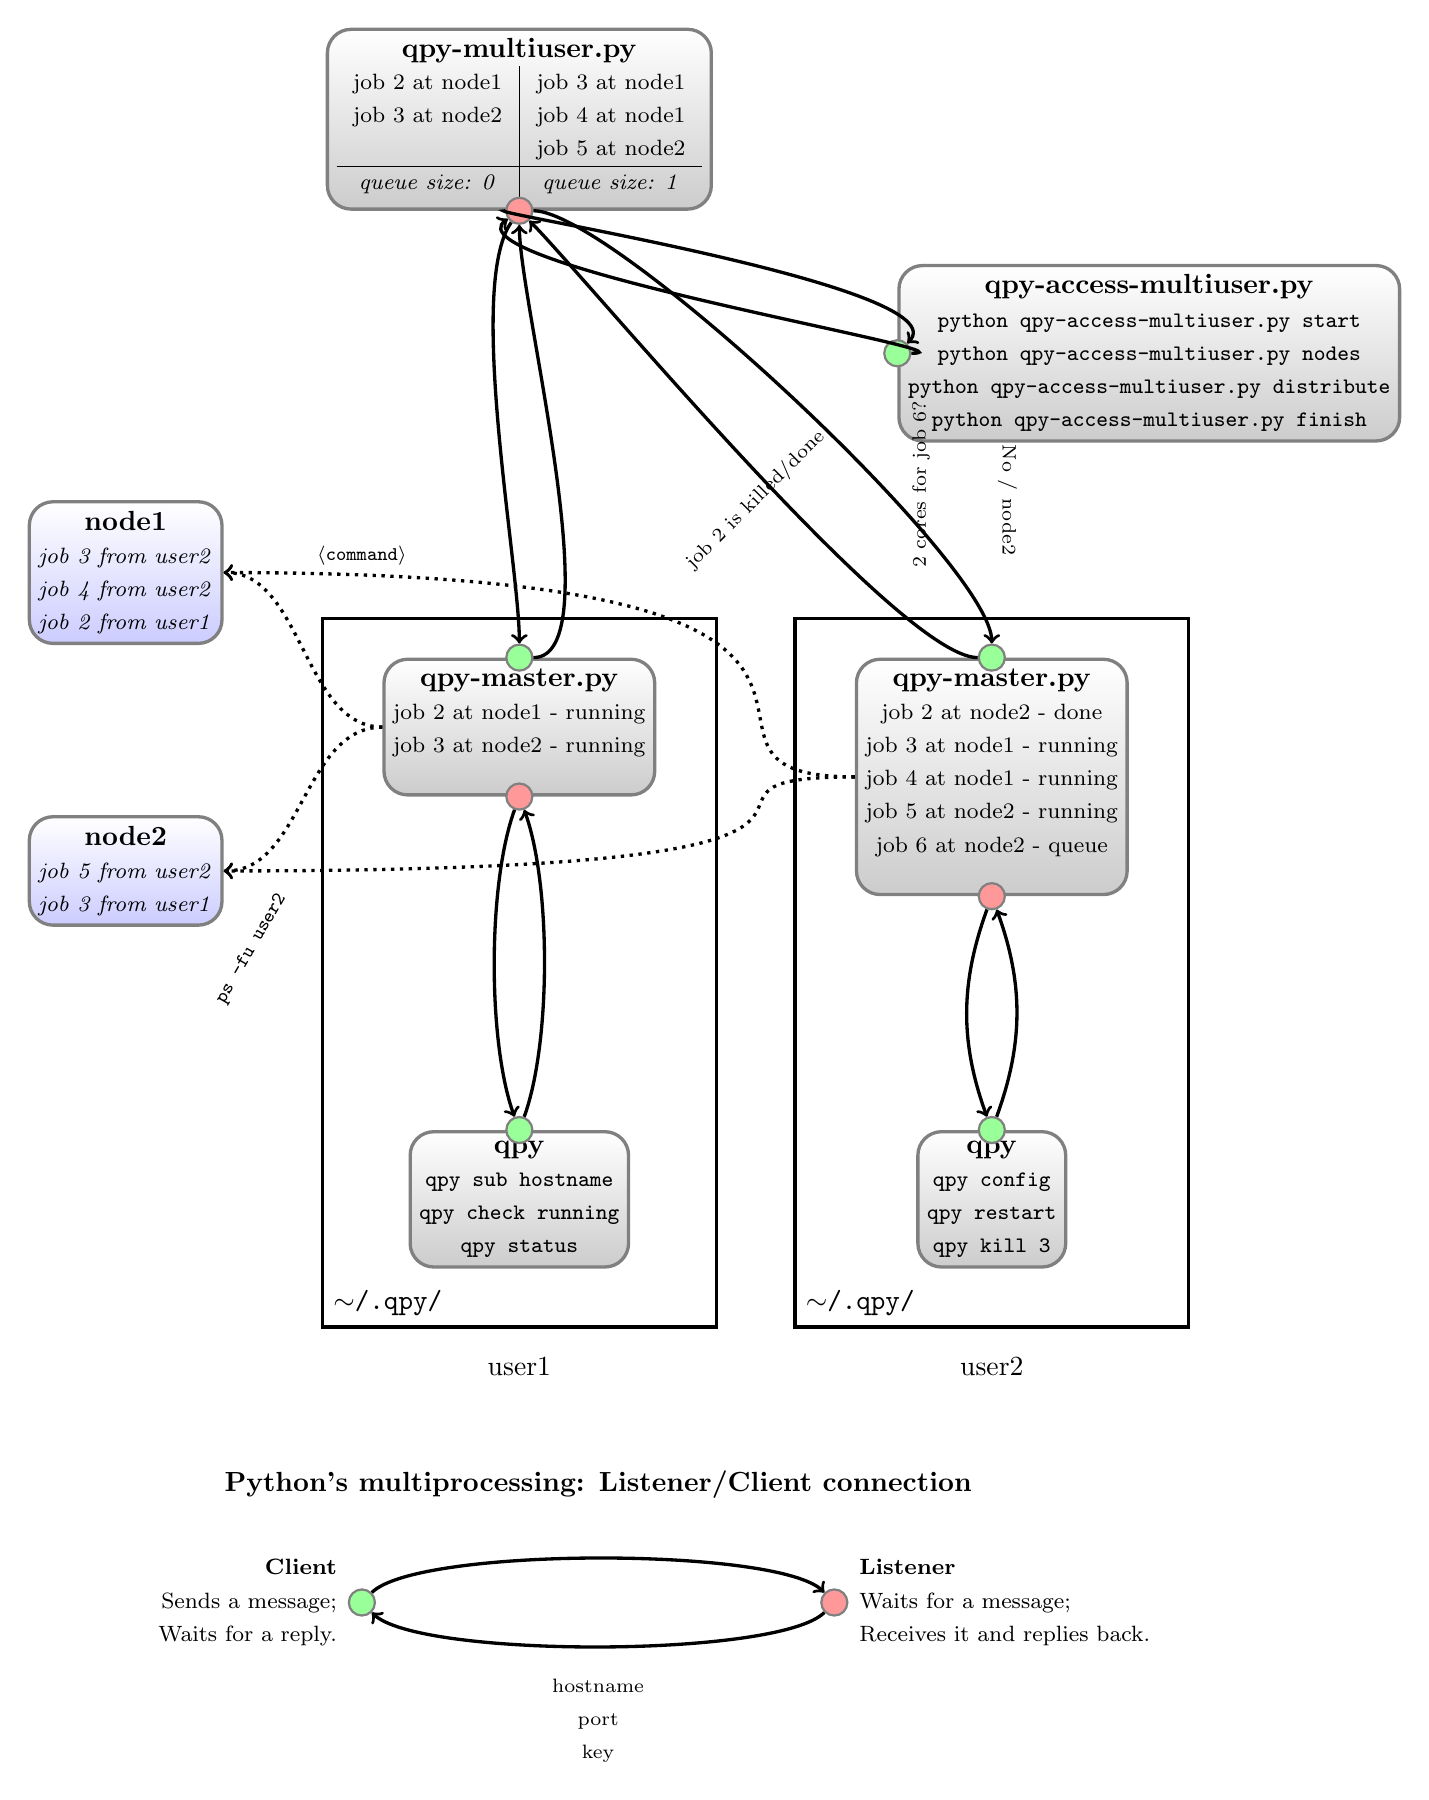
\begin{tikzpicture}[
    ->,
    double,
    very thick,
    program/.style={
      align=center, anchor=north,
      rectangle,minimum size=6mm,rounded corners=3mm,
      very thick,draw=black!50,
      top color=white,bottom color=black!20
    },
    comp/.style={
      align=center, anchor=north,
      rectangle,minimum size=6mm,rounded corners=3mm,
      very thick,draw=black!50,
      top color=white,bottom color=blue!20
    },
    list/.style={
      align=center, anchor=center,
      circle,minimum size = 0.3cm,
      thick,draw=black!50,
      fill=red!40
    },
    client/.style={
      align=center, anchor=center,
      circle,minimum size = 0.3cm,
      thick,draw=black!50,
      fill=green!40
    }
    ]

    \node (multiuser)  at (-3.0,3.0)[program] {
      \textbf{qpy-multiuser.py}\\
      \begin{tabular}{c|c}
        {\footnotesize job 2 at node1} & {\footnotesize job 3 at node1}\\
        {\footnotesize job 3 at node2} & {\footnotesize job 4 at node1}\\
        &{\footnotesize job 5 at node2}\\
        \hline
        \textit{\footnotesize queue size: 0}&\textit{\footnotesize queue size: 1}
      \end{tabular}
    };
    \node (multiuser_list) at (multiuser.south) [list] {};

    \node (access)  at (5.0,0.0)[program] {
      \textbf{qpy-access-multiuser.py}\\
      \texttt{\footnotesize python qpy-access-multiuser.py start}\\
      \texttt{\footnotesize python qpy-access-multiuser.py nodes}\\
      \texttt{\footnotesize python qpy-access-multiuser.py distribute}\\
      \texttt{\footnotesize python qpy-access-multiuser.py finish}
    };
    \node (access_client) at (access.west) [client] {};

    \draw [->] (multiuser_list.180) .. controls ++(180:0.4) and ++(45:1) .. (access_client.45);
    \draw [->] (access_client.0) .. controls ++(0:1) and ++(+215:1) .. (multiuser_list.215);

    \node (master1)  at (-3.0,-5.0)[program] {
      \textbf{qpy-master.py}\\
      {\footnotesize job 2 at node1 - running}\\
      {\footnotesize job 3 at node2 - running}\\
    };
    \node (master1_client) at (master1.north) [client] {};
    \node (master1_list) at (master1.south) [list] {};

    \draw [->] (master1_client.0) .. controls ++(0:1) and ++(-90:1) .. (multiuser_list.-90);
    \draw [->] (multiuser_list.+235) .. controls ++(+235:1) and ++(+90:1) .. (master1_client.90);
    
    \node (master2)  at (3.0,-5.0)[program] {
      \textbf{qpy-master.py}\\
      {\footnotesize job 2 at node2 - done}\\
      {\footnotesize job 3 at node1 - running}\\
      {\footnotesize job 4 at node1 - running}\\
      {\footnotesize job 5 at node2 - running}\\
      {\footnotesize job 6 at node2 - queue}\\
    };
    \node (master2_client) at (master2.north) [client] {};
    \node (master2_list) at (master2.south) [list] {};

    \draw [->] (master2_client.180) .. controls ++(180:1) and ++(-45:1) .. (multiuser_list.-45);
    \draw [->] (multiuser_list.0) .. controls ++(0:1) and ++(+90:1) .. (master2_client.90);


    \node (qpy1)  at (-3.0,-11.0)[program] {
      \textbf{qpy}\\
      \texttt{\footnotesize qpy sub hostname}\\
      \texttt{\footnotesize qpy check running}\\
      \texttt{\footnotesize qpy status}
    };
    \node (qpy1_client) at (qpy1.north) [client] {};

    \node (qpy2)  at (3.0,-11.0)[program] {
      \textbf{qpy}\\
      \texttt{\footnotesize qpy config}\\
      \texttt{\footnotesize qpy restart}\\
      \texttt{\footnotesize qpy kill 3}
    };
    \node (qpy2_client) at (qpy2.north) [client] {};

    \node (node1)  at (-8.0,-3.0)[comp] {
      \textbf{node1}\\
      \textit{\footnotesize job 3 from user2}\\
      \textit{\footnotesize job 4 from user2}\\
      \textit{\footnotesize job 2 from user1}
    };

    \node (node2)  at (-8.0,-7.0)[comp] {
      \textbf{node2}\\
      \textit{\footnotesize job 5 from user2}\\
      \textit{\footnotesize job 3 from user1}
    };

    
    \draw [->] (qpy1_client.70) .. controls ++(70:1) and ++(-70:1) .. (master1_list.-70);
    \draw [->] (master1_list.-110) .. controls ++(-110:1) and ++(+110:1) .. (qpy1_client.110);
    
    \draw [->] (qpy2_client.70) .. controls ++(70:1) and ++(-70:1) .. (master2_list.-70);
    \draw [->] (master2_list.-110) .. controls ++(-110:1) and ++(+110:1) .. (qpy2_client.110);
    
    
    \node [rotate=45] at (0.0,-3.0) {\scriptsize job 2 is killed/done};
    \node [rotate=90] at (2.1,-2.8) {\scriptsize 2 cores for job 6?};
    \node [rotate=-90] at (3.2,-3.0) {\scriptsize No / node2};
 
    \node at (-5,-3.7) {\texttt{\scriptsize $\langle$command$\rangle$}};
    \node [rotate=60] at (-6.4,-8.7) {\texttt{\scriptsize ps -fu user2}};

    \draw [->,dotted] (master1.-180) .. controls ++(-180:1) and ++(0:1) .. (node1.0);
    \draw [->,dotted] (master1.-180) .. controls ++(-180:1) and ++(0:1) .. (node2.0);
    \draw [->,dotted] (master2.-180) .. controls ++(-180:3) and ++(0:10) .. (node1.0);
    \draw [->,dotted] (master2.-180) .. controls ++(-180:3) and ++(0:10) .. (node2.0);
    
    
    \draw [] (-5.5, -4.5) rectangle (-0.5,-13.5);
    \draw [] (0.5, -4.5) rectangle (5.5,-13.5);
    \node [anchor=west] at (-5.5,-13.2) {$\sim$\texttt{/.qpy/}};    
    \node [anchor=west] at (0.5,-13.2) {$\sim$\texttt{/.qpy/}};    
    \node at (-3.0,-14.0) {user1};
    \node at (3.0,-14.0) {user2};
    
    
    
    \node at (-2.0,-15.5) {\textbf{Python's multiprocessing: Listener/Client connection}};
    \node [align=center] at (-2.0,-18.5) {\scriptsize hostname\\\scriptsize port\\\scriptsize key};
    
    \node (client_templ) [client] at (-5.0,-17.0){};
    \node (list_templ) [list] at (1.0,-17.0){};
    \node [anchor=east, align = right] at (client_templ.west) {
      \textbf{\footnotesize Client}\\
      {\footnotesize Sends a message;}\\
      {\footnotesize Waits for a reply.}
    };
    \node [anchor=west, align = left] at (list_templ.east) {
      \textbf{\footnotesize Listener}\\
      {\footnotesize Waits for a message;}\\
      {\footnotesize Receives it and replies back.}
    };
    
    \draw [->] (client_templ) .. controls ++(45:1) and ++(135:1) .. (list_templ);
    \draw [->] (list_templ) .. controls ++(-135:1) and ++(-45:1) ..  (client_templ);
    






% Grid
     % \foreach \y in {-15,...,2} {
     %   \node at (-9,\y) {\y};
     %   \draw [-] [dotted] (-8.5,\y) -- (5.0,\y);
     % };
     % \foreach \x in {-5,...,5} {
     %   \node at (\x,-18.5) {\x};
     %   \draw [-] [dotted] (\x,-18.0) -- (\x,2);
     % };
    

    
  \end{tikzpicture}
\end{center}

\linespread{1.5}



\end{document}

%%% Local Variables:
%%% ispell-local-dictionary: "british"
%%% mode: latex
%%% TeX-master: t
%%% End: 
